Temporary imports...

\begin{figure}[tbh]
  \begin{center}
    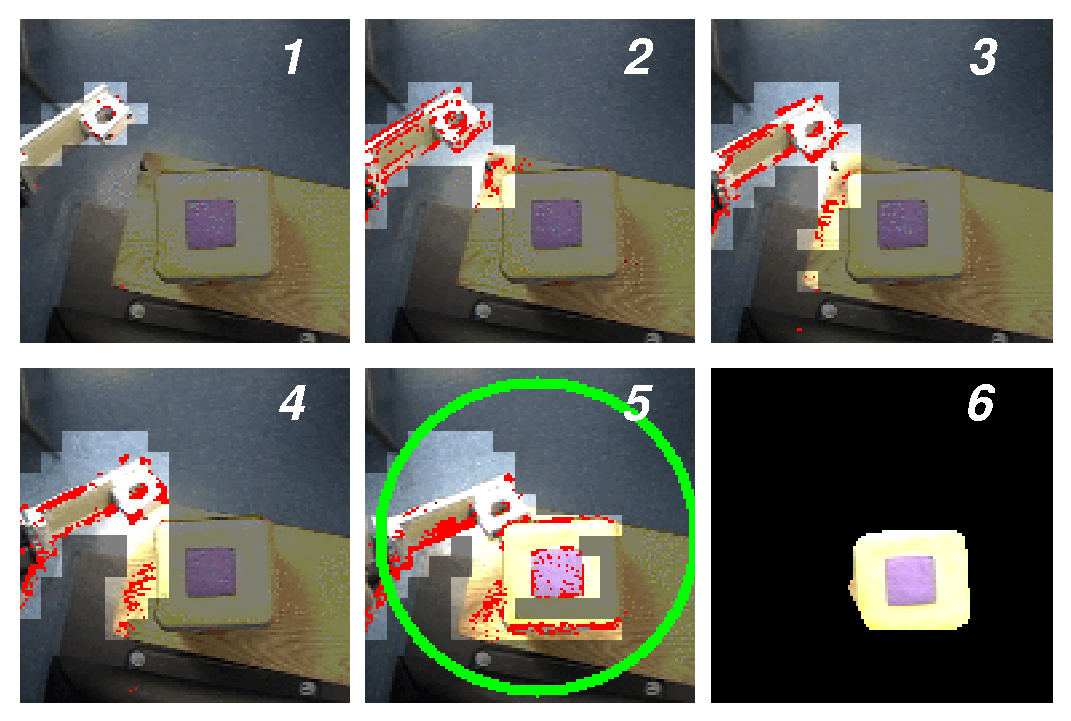
\includegraphics[width=12cm]{collision-detail}
  \end{center}
  \caption{
    The moment of impact is detected visually by the
    sudden expansion of motion away from the arm.  Motion before and
    after contact is compared to gather information for segmentation.
}
\end{figure}

\begin{figure}[tbh]
  \centerline{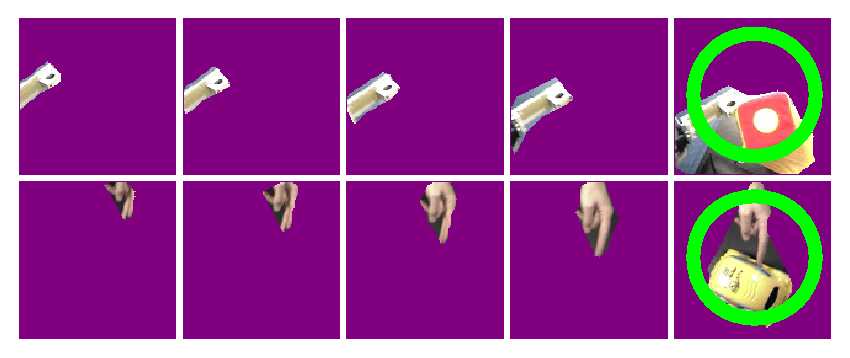
\includegraphics[width=12cm]{manipulator-segment}}
  \caption{Early experiments on segmenting the robot arm, or a 
human hand poking an object the robot is familiar with, by working
backwards from a collision event.}
  \label{fig:manipulator}
\end{figure}

\begin{figure}[tbh]
  \centerline{
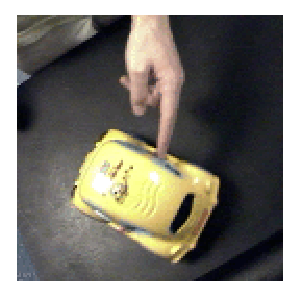
\includegraphics[width=5cm]{fig-car-hand-seg-src}
\hspace{1cm}

\includegraphics[width=5cm]{fig-car-hand-seg}
}
  \caption{A poke by hand}
  \label{fig:handpoke}
\end{figure}
